\chapter{Numerical Experiments} 
\label{ch:experiments}

In this section we analyze the empirical performance of OGD, comparing it with the algorithm from the Online Portfolio Optimization literature. We compare it to OLU~\cite{das2013online}, since it provides guarantees on total regret as described in Section \ref{sec:OLU}.
We also consider UP~\cite{cover1996universal} and ONS~\cite{agarwal2006algorithms}.
We selected UP (Section \ref{sec:UP}) because it has the best theoretical guarantees on the regret $R_T$, and ONS (Section \ref{sec:ONS}) because it has good theoretical guarantees on the regret $R_T$.\footnote{
We used a na\"ive version of UP since the classic implementation required an unfeasible amount of time for the experiments.
Instead, we discretized the simplex with $10^4$ points and used the corresponding CRPs to approximate the integrals used by UP.} ONS is also known to provide good empirical results on the regret $R_T$ when analyzed empirically.

\begin{table}[ht!]\centering\small
\begin{tabular}{ |c||c|c|c|c| }
 \hline
 \multicolumn{5}{|c|}{Datasets} \\
 \hline
 Name & Market &Year Span & Days & Assets\\
 \hline
 NYSE(O) & New York Stock Exchange  & 1962 - 1984  &5651&   36\\
 TSE & Toronto Stock Exchange & 1994 - 1998  & 1258   &88\\
 SP500 & Standard Poor's 500 & 1998 - 2003 & 1276&  25\\
 \hline
\end{tabular}
\caption{Description of the main datasets used commonly in the Online Portfolio Optimization literature.}\label{tab:dataset}
\end{table}

Table \ref{tab:dataset} summarizes the datasets used for the experiments. All the assets in the datasets have been anonymized to avoid common bias toward specific assets.
To compare the algorithms with previous results in the field we selected the NYSE(O) dataset, a well-known benchmark that has been previously used in several portfolio optimization research papers, and notably, in all the works which propose the algorithms considered here as baselines.
The NYSE(O) dataset spans $22$ years (between $1962$ and $1984$), for a total investment horizon of $T = 5651$ days ($\approx250$ working days per year).
In each experiment, we sampled a set of $N=5$ assets randomly chosen among the $36$ and ran the algorithms for the entire investment horizon $T$.
We ran $100$ independent experiments for the NYSE(O) dataset, $50$ and $50$ for the TSE and SP500 dataset respectively, and, then, we averaged the results. The choice of doing a larger number of experiments is to stress the point that we are not concerned with the selection of assets to invest in, but only with the behavior of the algorithms with respect to transaction costs.
We considered different values for the transaction rate $\gamma \in \{ 0, 0.0005, 0.001, 0.003, 0.006, 0.01, 0.02, 0.04 \}$, including large values of $\gamma$ to simulate highly illiquid markets.

To set the parameter $K$ of OGD we used the learning rate $\eta_t$ prescribed by Theorem~\ref{thm:total_regret}, with $\epsilon_l = 0.8$ and $\epsilon_u = 1.2$, for which Assumption~\ref{ass:nojunk} holds in the dataset NYSE(O).
For ONS, we used $\eta = 0$, $\beta = 1$, $\delta = 1/8$, as suggested by the authors in~\cite{agarwal2006algorithms}.
We used $\alpha = 0.12$ and $\eta = 1.3$ for OLU, which is the best combination of parameters according to~\cite{das2013online}.
All algorithms have been initialized with $\mathbf{x}_1 = \frac{1}{N} \mathbf{1}$.

We used the Annual Percentage Yield (APY) as a metric, assuming $250$ working days per year and one update per day.
Formally, the APY for the wealth $W$ is defined as:
\begin{equation*}
    A(W) = W^{250/T} - 1,
\end{equation*}
where $W \in \{ W_T^C, \tilde W_T \}$ which are defined in Equation \eqref{eq:l1_wealth} and \eqref{eq:realwealth} respectively.
$95\%$ confidence intervals for the mean have been computed with statistical bootstrapping and are depicted as semi-transparent areas.

\section{Results on the NYSE(O) dataset}

\begin{figure}[ht!]
    \centering
    \subfloat[\label{fig:ex1}]{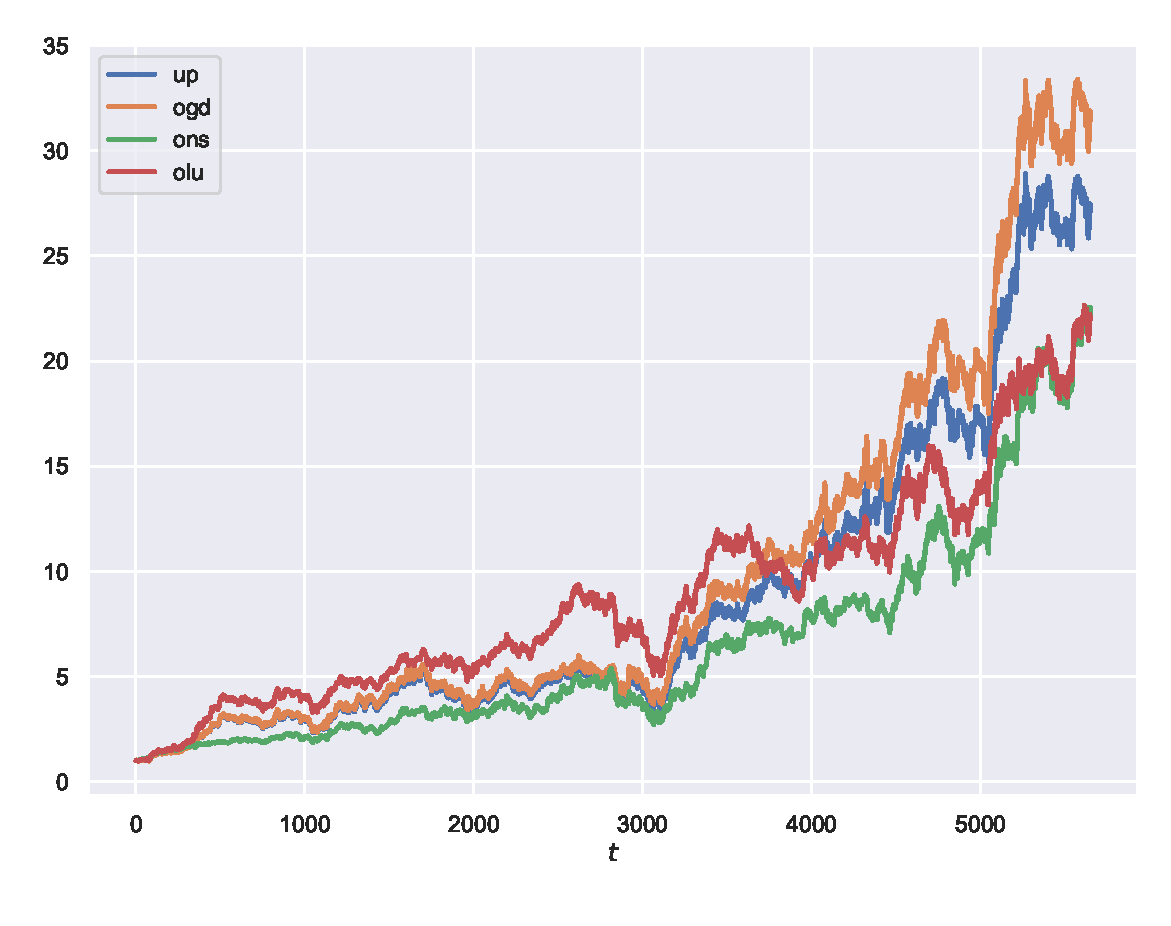
\includegraphics[width=0.48\textwidth,keepaspectratio]{img/fig_11.pdf}}
    \subfloat[\label{fig:ex2}]{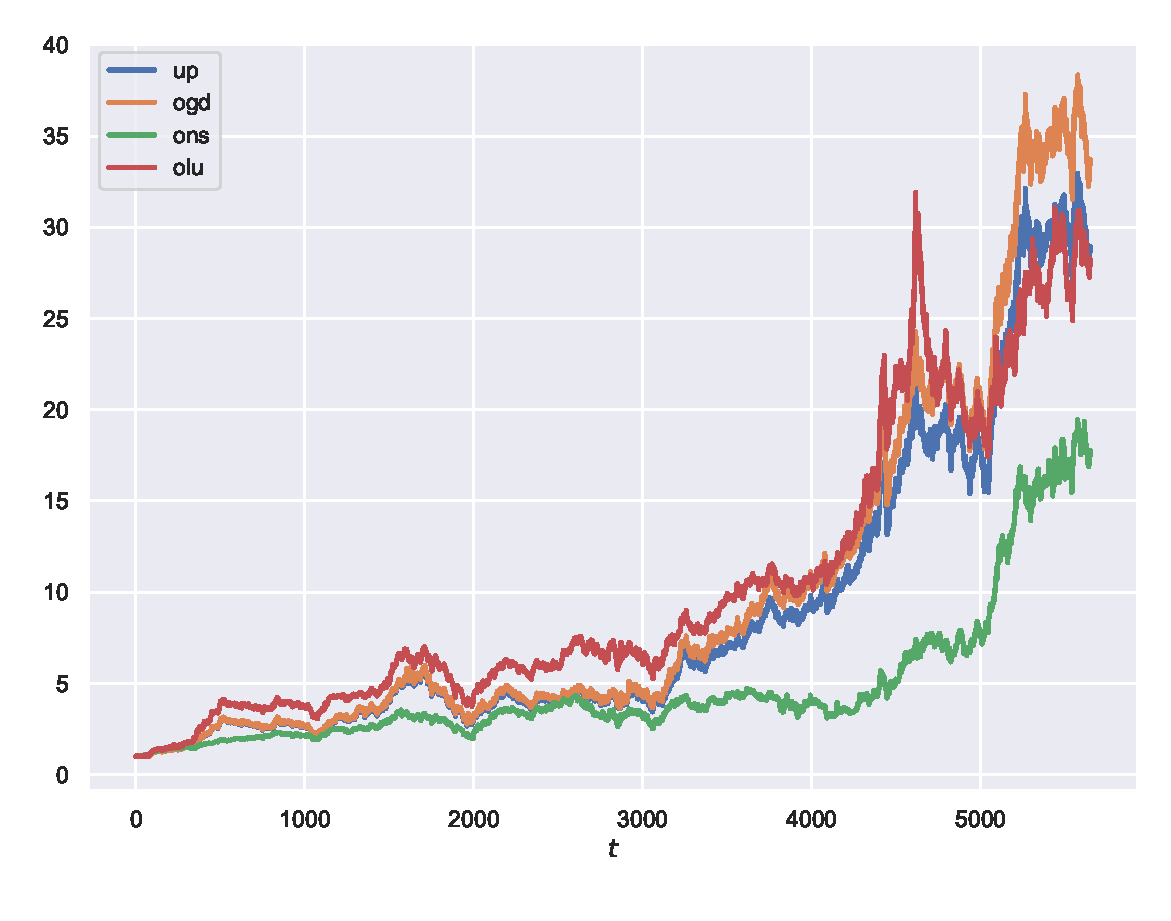
\includegraphics[width=0.48\textwidth,keepaspectratio]{img/fig_12.pdf}}
\caption{Wealth $W_T^C(\mathcal{A})$ on two runs of the NYSE(O) for $\gamma = 0$ (a), and $\gamma = 0.001$ (b).} \label{fig:algo_copmarison}
\end{figure}

Figure~\ref{fig:algo_copmarison} shows the evolution of the total wealth ${W}^C_t(\mathcal{A})$ of the different algorithms over the investment horizon in two specific runs, one without any cost ($\gamma = 0$) (Figure~\ref{fig:ex1}), and one with a transaction rate of $\gamma = 0.001$ (Figure~\ref{fig:ex2}).
In these two specific runs, OGD obtains a cumulative wealth larger than any other algorithm analyzed, suggesting that, in some settings, it might provide the best performance.
The results with $\gamma = 0$ suggest that OGD might be a viable solution even in the absence of costs.


\begin{figure}[ht!]
\centering
{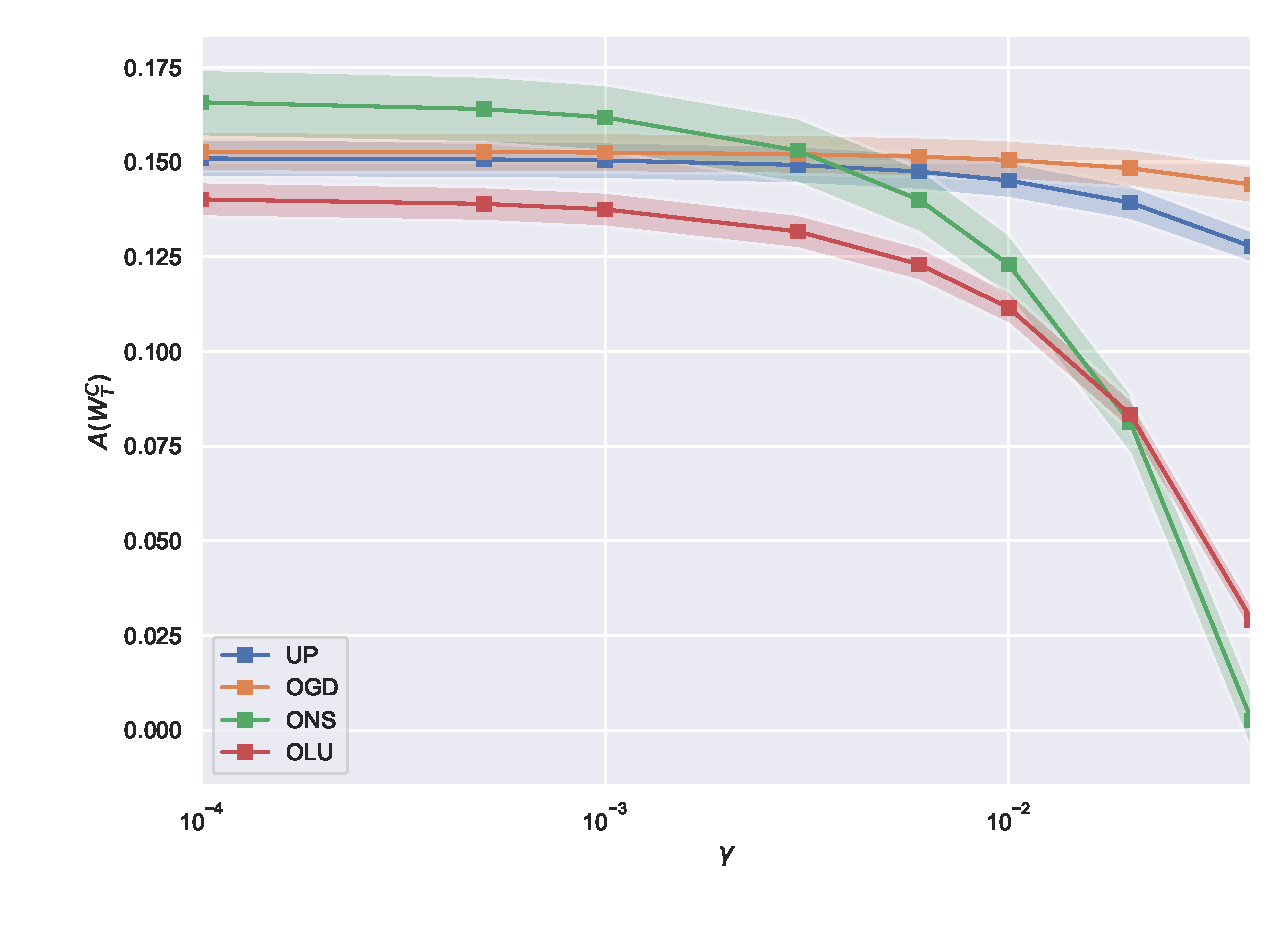
\includegraphics[width=0.70\textwidth,keepaspectratio]{img/fig_w_decay_l1.pdf}} 
\caption{Average APY computed on the wealth $W_T^C$ assuming the costs given by $C_T(\mathcal{A})$ for the NYSE(O) dataset.}
\label{fig:wealth_decay_l1}
\end{figure}

\begin{figure}[ht!]
\centering
{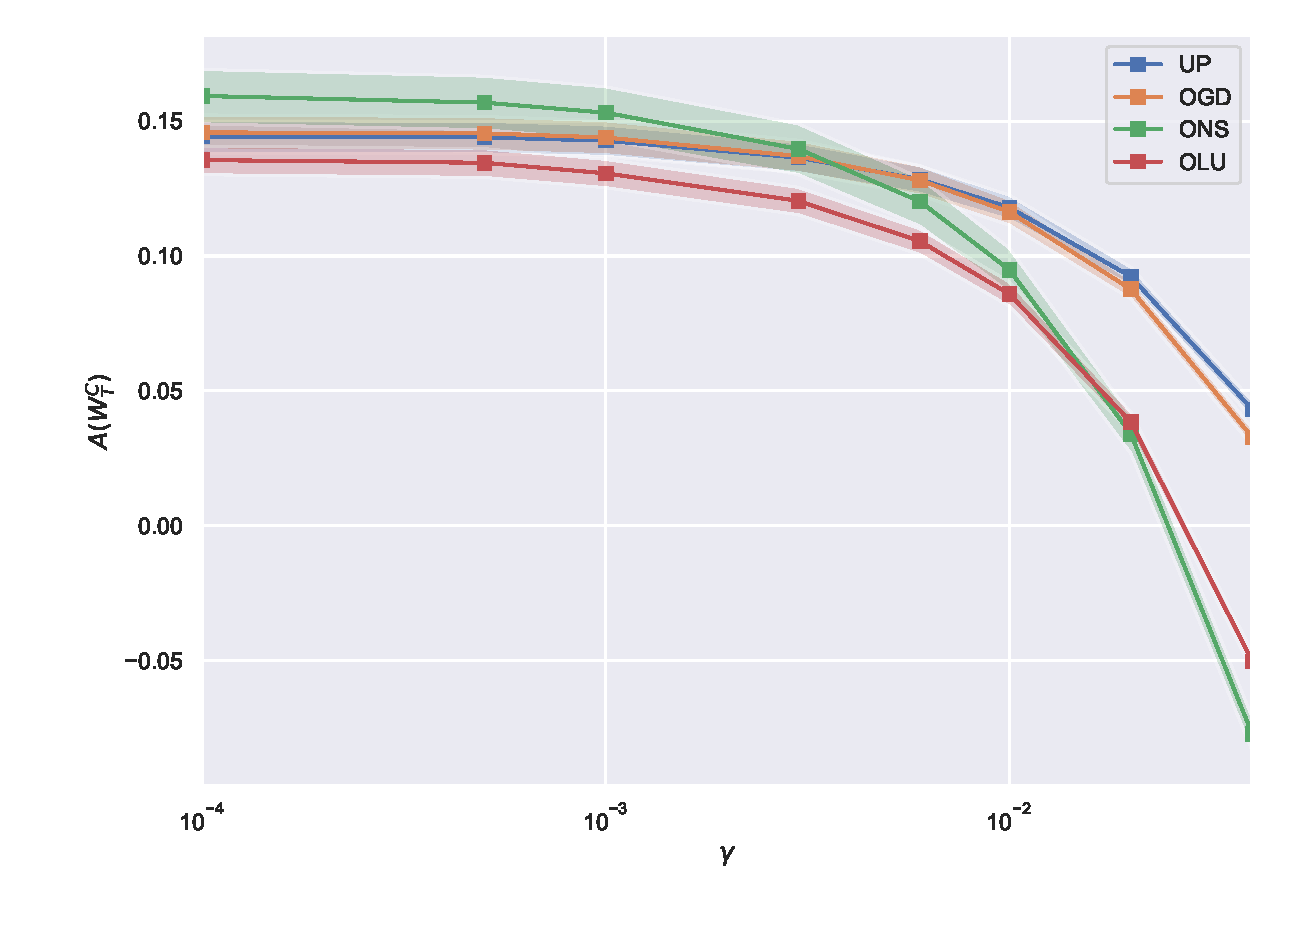
\includegraphics[width=0.70\textwidth,keepaspectratio]{img/fig_w_decay_true.pdf}} 
\caption{ Average APY computed on the wealth $\tilde{W}_T(\mathcal A)$ assuming the costs given by Equation~\eqref{eq:real_tc}, for the NYSE(O) dataset.}
\label{fig:wealth_decay_true}
\end{figure}

\begin{figure}[ht!]
\centering
{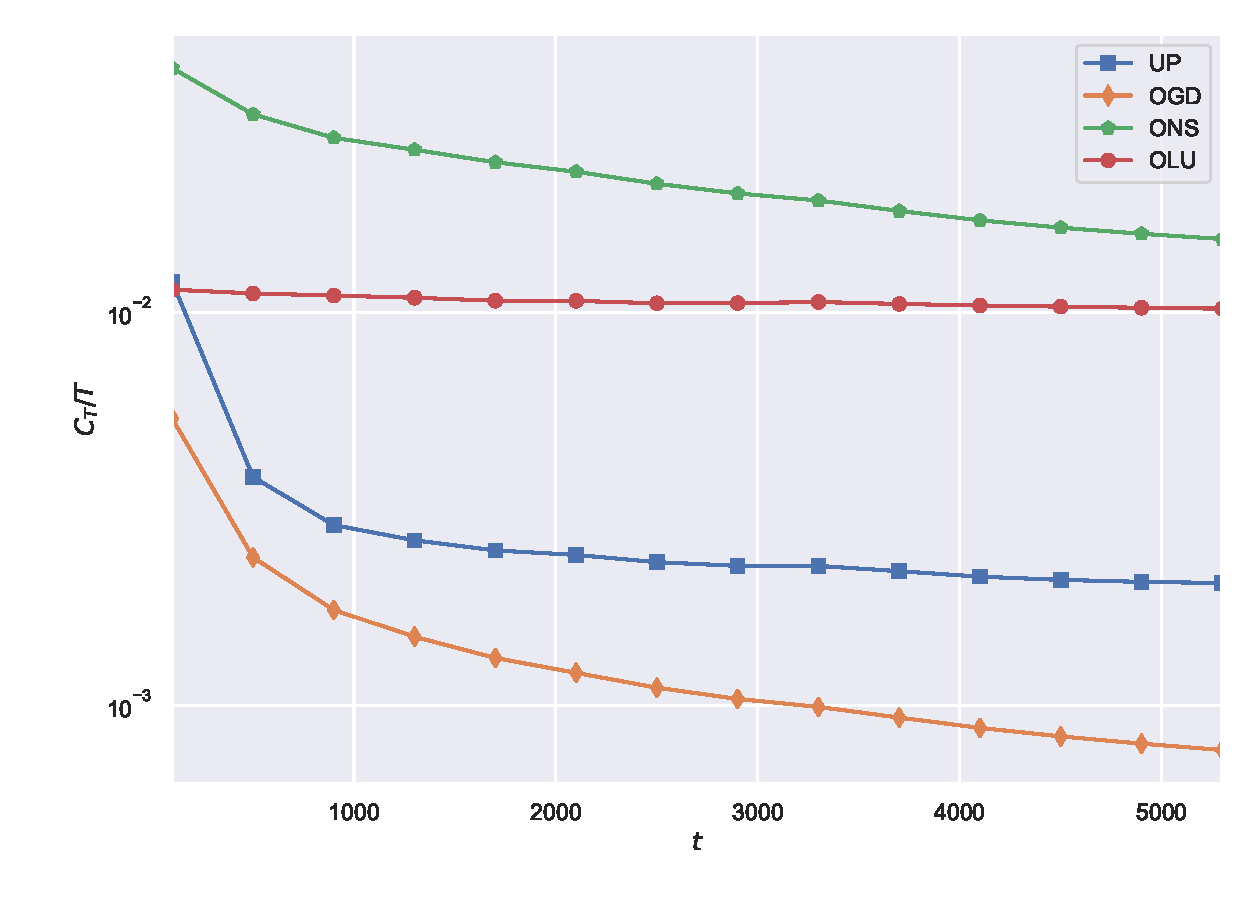
\includegraphics[width=0.70\textwidth,keepaspectratio]{img/fig_costs.pdf}}
\caption{Average costs $C_T(\mathcal{A})$ with $\gamma = 1$, for the NYSE(O) dataset.}
\label{fig:costs}
\end{figure}

In Figure~\ref{fig:wealth_decay_l1} we present the results for the average APY, with the corresponding confidence intervals.
In particular, with no transaction costs ($\gamma = 0$), all the analyzed algorithms give similar results.
In this setting, ONS is the algorithm with the largest APY.
As we increase the transaction rate $\gamma$, OGD gets the largest APY, while OLU and ONS seem to be penalized by large transaction costs.
Conversely, the fact that the APY decreases from $\approx 0.15$ to $\approx 0.14$ suggests that OGD is effective at minimizing the costs $C_T(\mathcal{A})$.

Figure~\ref{fig:wealth_decay_true} considers the wealth $\tilde{W}_T(\mathcal{A})$, \emph{i.e.}, the one defined in Equation~\eqref{eq:realwealth}.
We notice that, comparing these results with the ones obtained using $W_T^C$ (Figure~\ref{fig:wealth_decay_l1}), we have a smaller APY when $\gamma \gg 0$.
This suggests that, when applied to real-world cases, they might under-perform w.r.t.~what is expected from the theoretical results. 
In terms of $\tilde{W}_T(\mathcal{A})$, UP seems to perform slightly better than OGD, but the difference is not statistically significant for $\gamma < 0.04$.
ONS and OLU provide negative profits ($A(\tilde{W}_T) < 0$) for large values of transaction costs, \emph{e.g.}, for $\gamma = 0.04$ the APY becomes negative and, thus, the accumulated wealth is completely canceled out by the transaction costs.
From Figure~\ref{fig:wealth_decay_true} we would be inclined to choose ONS for $\gamma \leq 0.003$, and OGD for $\gamma \geq 0.003$.

Figure~\ref{fig:costs} shows the averaged cost per round $C_t(\mathcal{A})/t$ and the corresponding confidence intervals, with $\gamma = 1$ (the value of $\gamma$ has been chosen to easily interpret how the regret on the costs behaves over time).
OGD is the algorithm that provides the lowest cost per round, which strengthens the claim of this work that OGD keeps transaction costs low.
The costs per round for OLU are approximately linear, as expected from the theory (see Section~\ref{sec:OLU}).
Conversely, the results for ONS, while not having any theoretical guarantee on $C_T(\mathcal{A})/T$, suggest that it has a cost per round of order $\mathcal{O}(\sqrt{T})$, but with a larger constant than OGD.
Finally, the costs of UP decrease slower than those of ONS and OGD.

\subsection{Results on the TSE and SP500 dataset}

\begin{figure}[ht!]
\centering
{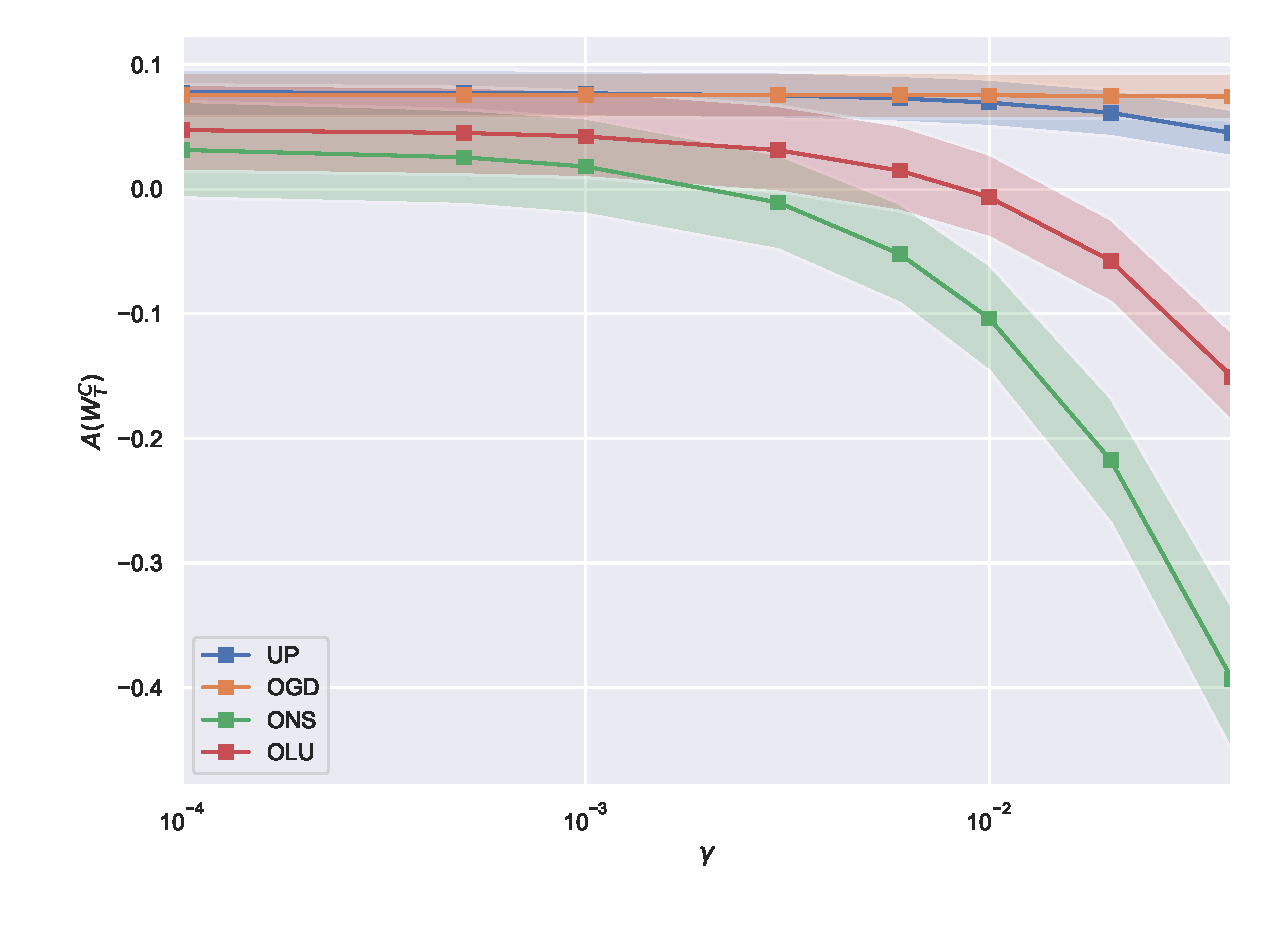
\includegraphics[width=0.70\textwidth,keepaspectratio]{img/fig_w_decay_l1_tse.pdf}} 
\caption{Average APY computed on the wealth $W_T^C$ assuming the costs given by $C_T(\mathcal{A})$ for the TSE dataset.}
\label{fig:wealth_decay_l1_tse}
\end{figure}

\begin{figure}[ht!]
\centering
{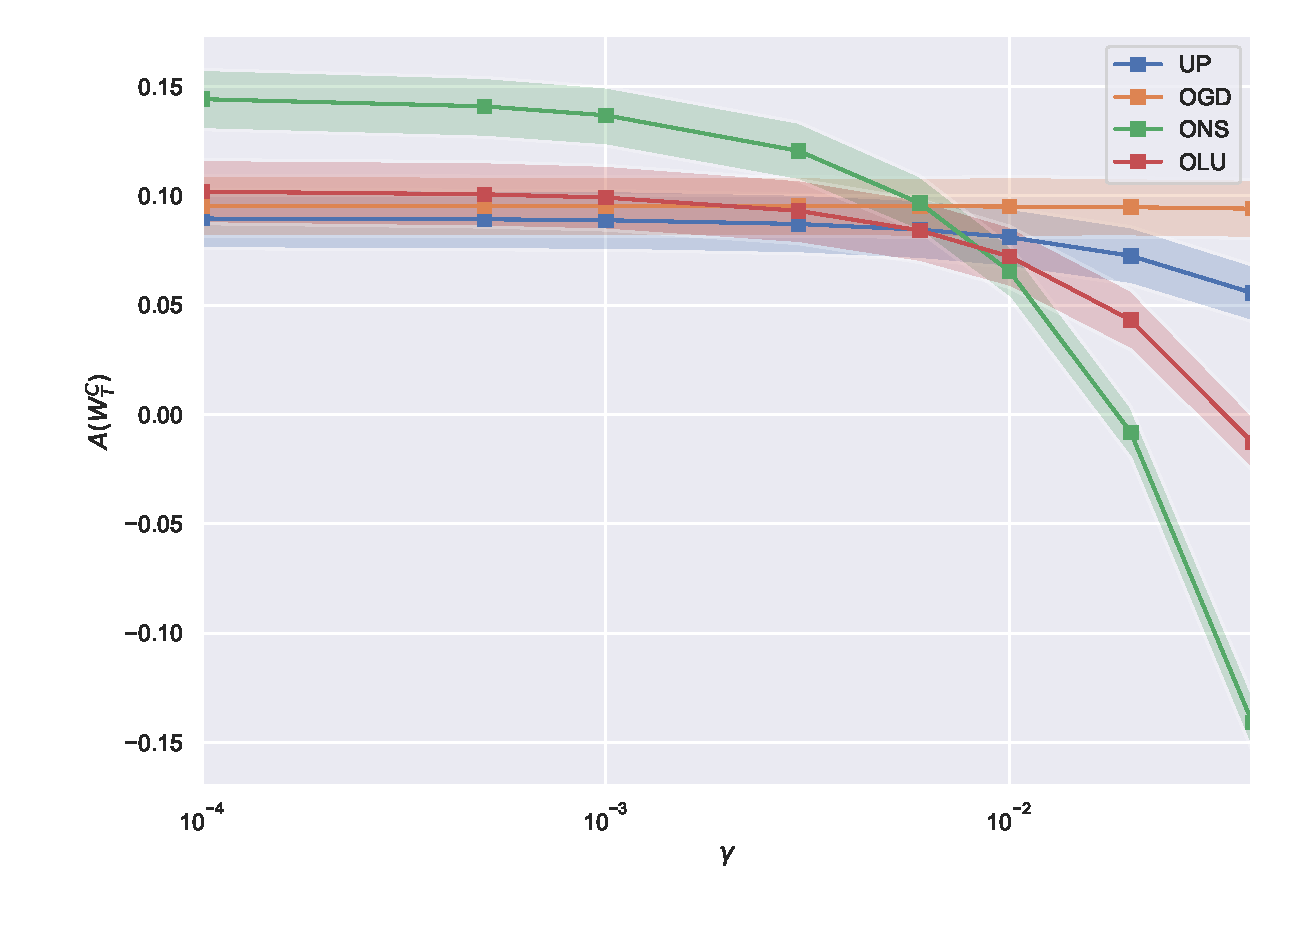
\includegraphics[width=0.70\textwidth,keepaspectratio]{img/fig_w_decay_l1_sp500.pdf}} 
\caption{Average APY computed on the wealth $W_T^C$ assuming the costs given by $C_T(\mathcal{A})$ for the SP500 dataset.}
\label{fig:wealth_decay_l1_sp500}
\end{figure}

In Figure \ref{fig:wealth_decay_l1_tse} and \ref{fig:wealth_decay_l1_sp500} we present the results obtained on the TSE and SP500 datasets respectively, using the same approach we used for the NYSE(O) dataset.  The results obtained are in line with the one presented with the NYSE(O) dataset, \emph{i.e.}, the OGD algorithm performs better than the others for transaction rate greater than $0.003$, while it presents similar performance, in terms of APY, for smaller values of the transaction rate. Notably, in the SP500 dataset, ONS outperforms the other algorithms for small transaction rate $\gamma$, while in the TSE dataset, it is out-performed by the other algorithms, even for small values of the transaction rate $\gamma$.

\section{Results on the Custom Dataset}

For the experiments carried out in this section, we collected a new dataset to test further the algorithms.

\begin{table}[ht!]\centering
\begin{tabular}{ |c||c|c| }
 \hline
 \multicolumn{3}{|c|}{Custom Data (03/29/2019 - 03/29/2020)} \\
 \hline
 Ticker & Description & Market Category\\
 \hline
 SPY & SPDR S\&P 500 ETF Trust (SPY)  & Equity\\
 BNDX &  Vanguard Bond Index Fund ETF & Fixed Income\\
 DAX & Global X DAX Germany ETF & Equity\\
 VIX & CBOE Volatility Index & Derivatives\\
 \hline
\end{tabular}
\caption{Detailed description of the custom dataset.}\label{tab:dataset_custom}
\end{table}

Table \ref{tab:dataset_custom} gives a description of the tailored dataset. We used data for one year (from April 2019 to April 2020), including the period of December 2019 - March 2020 that shows a global decline in the global financial markets. We included two Equity indices (SPY and DAX) as a proxy for the USA markets and European markets, then we included a Bond index (BNDX) and a volatility index (VIX) that simulate a Variance Swap, that allows investor to profit from volatility in the markets \cite{bossu2006introduction}.

We are well aware that a back-testing procedure not rigid enough can lead to over-fitting and biased results, which is an important problem in the financial literature (\cite{bailey2016probability}, \cite{harvey2015backtesting}).
Nonetheless, we found interesting to present these results, as these not only confirm the findings of the previous section, but also give insight on the inner workings of the algorithms. 

To set the parameters of ONS and OLU for the experiments performed on this dataset we used as a validation the first $1/4$ of the dataset (corresponding approximately to the first $3$ months of the dataset), performed  grid search algorithm and picked the parameters with the highest wealth $W_T$ on the validation set. The results of the grid search are presented in Figure \ref{fig:grid}. For the OGD algorithm we set the parameter $K$ to minimize the bound according to Theorem~\ref{thm:total_regret}.

\begin{figure}[ht!]
    \centering
    \subfloat[\label{fig:grdid_ONS}]{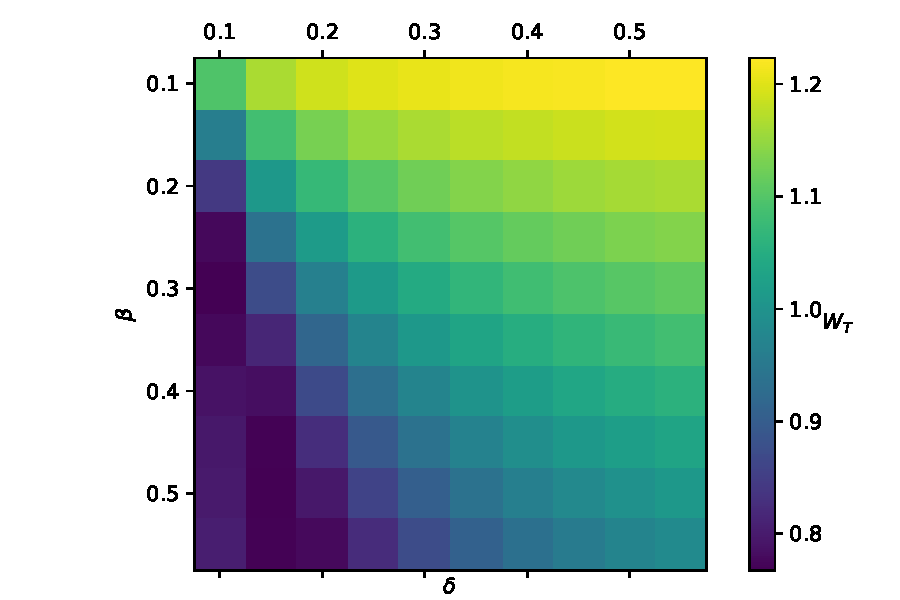
\includegraphics[width=0.48\textwidth,keepaspectratio]{img/grid_ONS.pdf}}
    \subfloat[\label{fig:grid_OLU}]{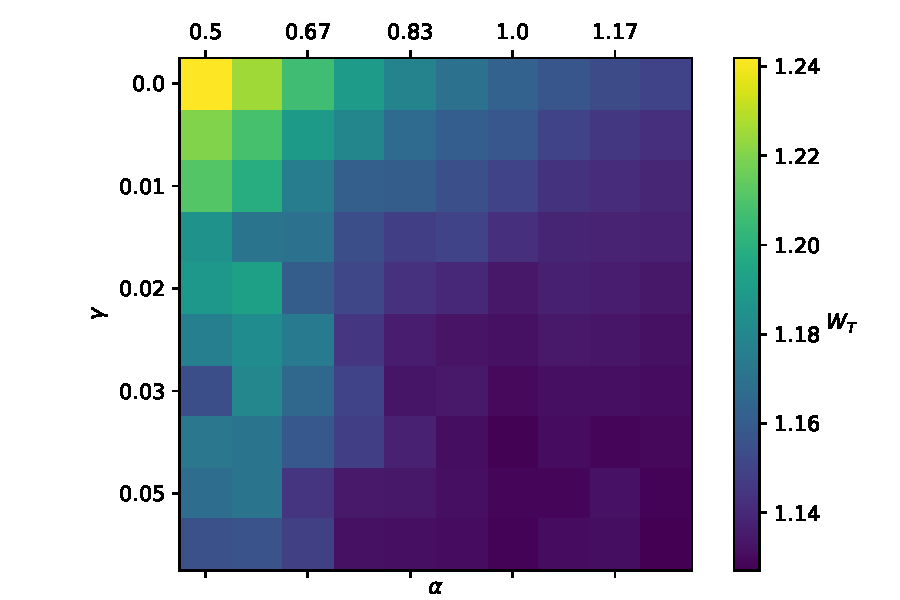
\includegraphics[width=0.48\textwidth,keepaspectratio]{img/grid_OLU.pdf}}
\caption{Grid search for the parameters of ONS (a) and OLU (b) on the validation set of the custom dataset.} \label{fig:grid}
\end{figure}

Figure \ref{fig:wealth_custom} shows the results for the algorithms run on the custom dataset. The transaction rate was set to $\gamma=0.001$ for all the algorithms. The reason why UP and OGD outperform the other two algorithms in this dataset, is the fact that they kept a larger portion of their allocation in the VIX index throughout the investment period. This lead to larger gains in the last two months. On the other hand ONS and OLU had nearly none of the VIX index in their allocations towards the end of the period, because it was performing poorly during the previous months. This lead to great losses in the last months of the trading period, due to the decrease of the other assets. 

In Figure \ref{fig:costs_custom} we show the dependency of the wealth achieved by algorithms to the transaction rate parameter $\gamma$ for the run on this dataset. We see how OGD shows a near constant wealth in relation to the transaction costs parameter $\gamma$, while UP only has a mild decline in wealth for large value of $\gamma$. Conversely, we see how ONS and OLU have a rapid decline in wealth w.r.t. the transaction rate $\gamma$.

\begin{figure}[ht!]
\centering
{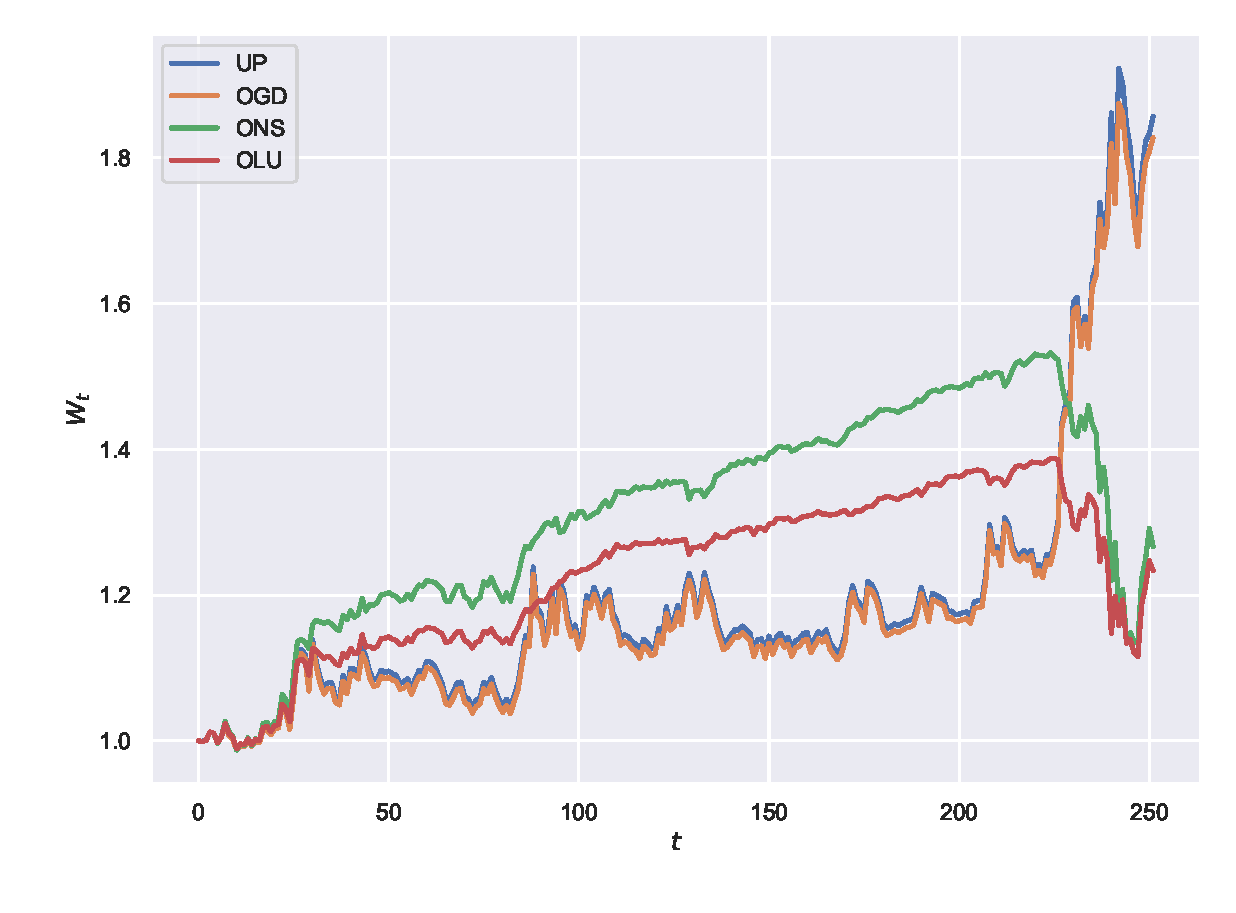
\includegraphics[width=0.70\textwidth,keepaspectratio]{img/new_experiemnts_1920.pdf}} 
\caption{Wealth $\tilde W_t$ achieved on the custom dataset described in Table \ref{tab:dataset_custom}, with $\gamma=0.001$.}
\label{fig:wealth_custom}
\end{figure}

\begin{figure}[ht!]
\centering
{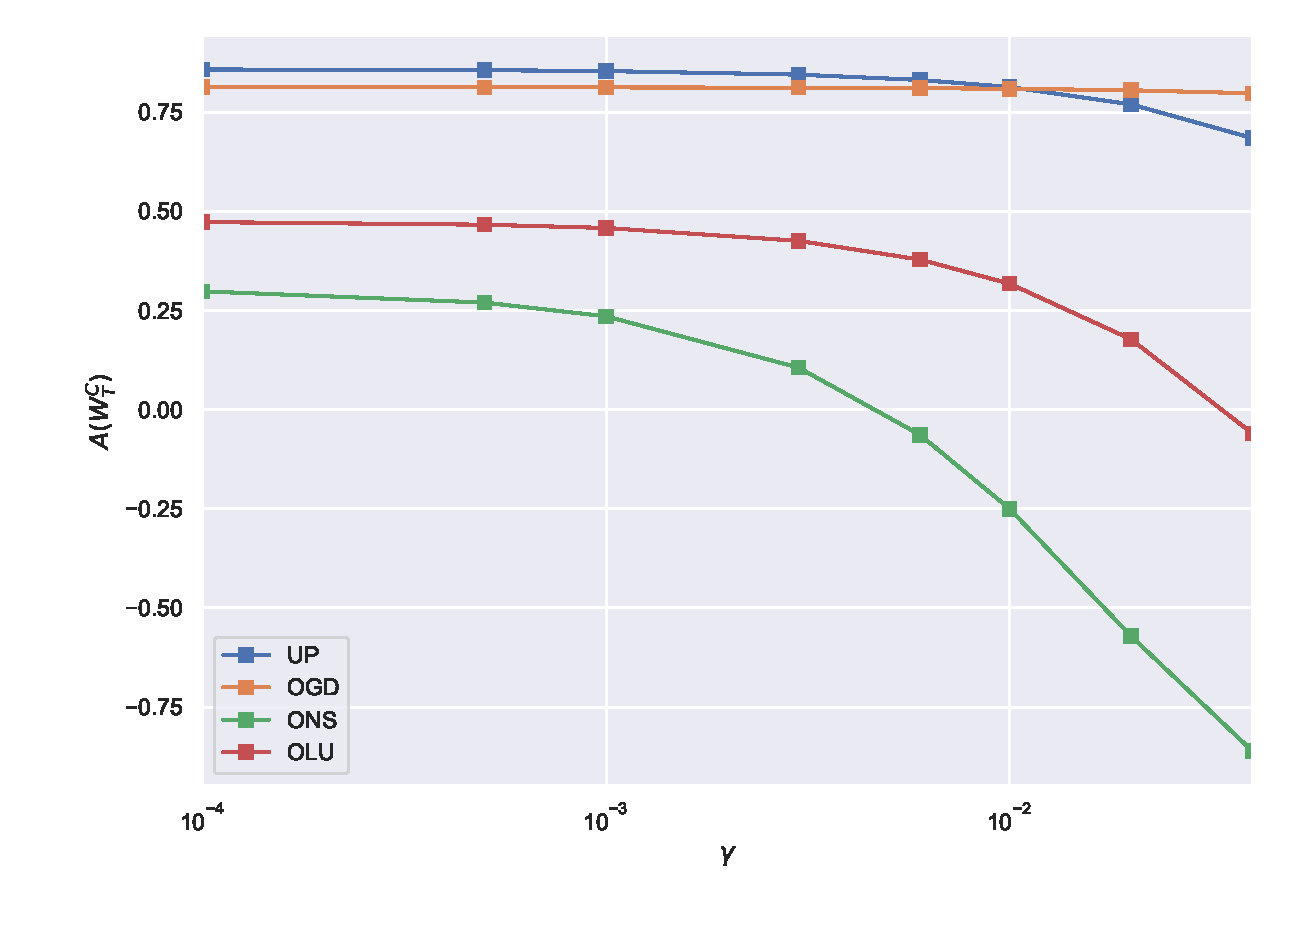
\includegraphics[width=0.70\textwidth,keepaspectratio]{img/new_experiemnts_1920_costs.pdf}} 
\caption{APY computed on the wealth $W_T^C(\mathcal A)$, assuming costs given by $C_T(\mathcal A)$ for the custom dataset.}
\label{fig:costs_custom}
\end{figure}
